\documentclass[12pt,a4paper,notitlepage,oneside,amsmath,amssymb]{article}
\usepackage{geometry}  % See geometry.pdf to learn the layout options. There are lots.
\geometry{a4paper, margin=1in, noheadfoot} % ... or a4paper or a5paper or ...
\usepackage[utf8]{inputenc}
\usepackage{graphicx}
\graphicspath{{./img/}}
\usepackage{amsmath}
\usepackage{amssymb}
% \usepackage{fontspec}
% \setromanfont{LiHei Pro}
% \XeTeXlinebreaklocale "zh"
% \XeTeXlinebreakskip = 0pt plus 1pt
\usepackage{CJKutf8}
\usepackage{anyfontsize}
\usepackage{caption}
\usepackage{indentfirst}
\usepackage{titlesec}
\usepackage{enumitem}
\usepackage[normalem]{ulem}
\usepackage[most]{tcolorbox}
% \tcbuselibrary{breakable}
% \usepackage{cancel}
\usepackage{xcolor}
% \usepackage[pages=all]{background}
\definecolor{text}{rgb}{0.1, 0.1, 0.1}
\color{black}

\titleformat*{\section}{\large\bfseries}
\titleformat*{\subsection}{\large\bfseries}
\titleformat*{\subsubsection}{\large\bfseries}
\titleformat*{\paragraph}{\large\bfseries}
\titleformat*{\subparagraph}{\large\bfseries}
% \titlespacing*{<command>}{<left>}{<before-sep>}{<after-sep>}
\titlespacing*{\section}{0pt}{15pt}{4pt}


% \setlength{\parindent}{0em}
% \setlength{\parskip}{0.5em}
% \setlength{\columnsep}{0.5cm}
\renewcommand{\baselinestretch}{1.2} % scales the default interline space to 1.5 its default value.

% \setlist[itemize]{topsep=2pt, itemsep=0.2ex, partopsep=0ex, parsep=0ex, nosep, leftmargin=3ex,
% labelindent=1ex, labelwidth=1ex}
% \setlist[enumerate]{topsep=2pt, itemsep=0.2ex, partopsep=0.5ex, parsep=0.2ex, nosep,
%     labelindent=2ex, labelwidth=2ex}

\begin{document}
\begin{CJK*}{UTF8}{bkai}

	\CJKtilde{}
	\CJKindent{}
	\title{\vspace{-10ex}DIP HW4 Report}
	\author{R07922036~邱能賢}
	\date{\vspace{-1ex}\today}

	\maketitle

	\vspace{-5ex}

	\section*{Problem 1: Hough Transform for Line Detection}

	\begin{enumerate}[label=(\alph*)]
		\item Perform edge detection on \(I_1\) and output the resultant edge map as \(E\).

		      I perform edge detection with Canny edge detector, the same method as in HW\#2.

		      \begin{figure}[hbt!]
			      \centering
			      \begin{minipage}{.4\textwidth}
				      \centering
				      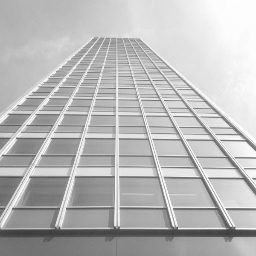
\includegraphics[width=.85\linewidth]{sample1}
				      \caption*{\(I_1\), sample1.raw}
			      \end{minipage}%
			      \begin{minipage}{.4\textwidth}
				      \centering
				      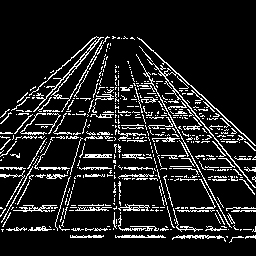
\includegraphics[width=.85\linewidth]{image_E}
				      \caption*{image \(E\) - edge map}
			      \end{minipage}
		      \end{figure}

		\item Perform Hough transform on \(E\) and output the accumulator array as a new image, \(H_1\), where the horizontal axis and vertical axis represent theta and rho values.

		      I set the accumulator array with a size of \(127\times127\), that is, quantize both \(\rho\) and \(\theta\) to 127 bins.

		\item Perform contrast adjustment on \(H_1\) and output the result as \(H_2\) for better visualization.

		      I perform global histogram equalization to do the contrast adjustment on \(H_1\), as in HW\#1.

		      \begin{figure}[hbt!]
			      \centering
			      \begin{minipage}{.4\textwidth}
				      \centering
				      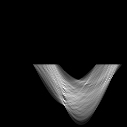
\includegraphics[width=.85\linewidth]{image_H1}
				      \caption*{\(H_1\)}
			      \end{minipage}%
			      \begin{minipage}{.4\textwidth}
				      \centering
				      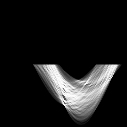
\includegraphics[width=.85\linewidth]{image_H2}
				      \caption*{\(H_2\)}
			      \end{minipage}
		      \end{figure}

		      \newpage

		\item By utilizing the accumulator array, draw the top 10 and top 20 significant lines with different colors on the edge map \(E\) and output the resultant images as \(D_1\) and \(D_2\).

		      I use an C++ \texttt{multimap}, which is implemented with a binary tree, to sort the accumulator array values. Then, find the top 10 or 20 \((\rho, \theta)\) coordinate. Each \((\rho, \theta)\) coordinate corresponds to a line on the image coordinate. The color of each line represents the order of their accumulated values. The red one is the most significant line, and the color turns blue as the  accumulated value decrease.

		      \begin{figure}[hbt!]
			      \centering
			      \begin{minipage}{.5\textwidth}
				      \centering
				      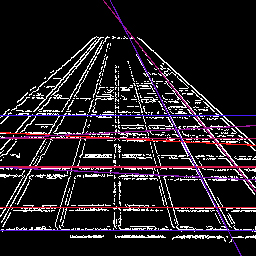
\includegraphics[width=.8\linewidth]{image_D1}
				      \caption*{\(D_1\)}
			      \end{minipage}%
			      \begin{minipage}{.5\textwidth}
				      \centering
				      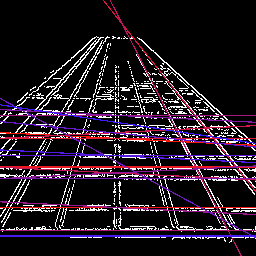
\includegraphics[width=.8\linewidth]{image_D2}
				      \caption*{\(D_2\)}
			      \end{minipage}
		      \end{figure}

		      Most lines did align with the edges, but because the edge map is not very clean, some lines are overlaying each other with only slight difference in angle. In \(D_2\), there are even some less significant lines that doesn't align with the edges.

		      I've also tried different Hough array size, and here are the result of image \(D_1\):

		      \begin{figure}[hbt!]
			      \centering
			      \begin{minipage}{.3\textwidth}
				      \centering
				      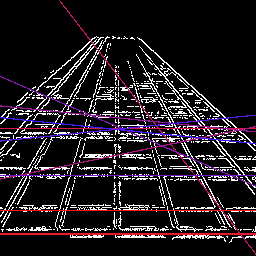
\includegraphics[width=.9\linewidth]{image_D1_63}
				      \caption*{size = 63}
			      \end{minipage}%
			      \begin{minipage}{.3\textwidth}
				      \centering
				      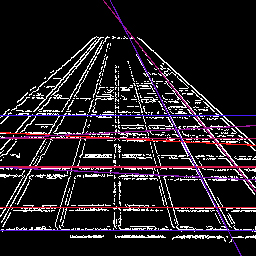
\includegraphics[width=.9\linewidth]{image_D1}
				      \caption*{size = 127}
			      \end{minipage}%
			      \begin{minipage}{.3\textwidth}
				      \centering
				      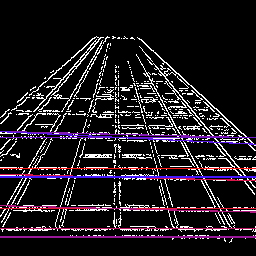
\includegraphics[width=.9\linewidth]{image_D1_255}
				      \caption*{size = 255}
			      \end{minipage}
			  \end{figure}

			  When the array size is too small, many edge map pixel will be accumulated at the same bin. Without enough ``resolution'', the lines doesn't match well with lines on the edge map. On the other hand, if the array size is too large, due to the unclean edge map, one noisy line may be quantized into multiple pixels. So in image \(D_1\) we can see that one edge will be split into many overlaying lines.

			  Hough transform is a very good method to detect lines or circles in an image, even if there are some discontinuity of the edges or background noise. But, as the discussion above showed, the result is highly affected by the quantization array size, so it must be chosen very carefully. Also, Hough transform is dependent on the quality of the edge map. The result will be much cleaner and accurate if the method of edge detection is improved.

	\end{enumerate}

	\clearpage

\end{CJK*}
\end{document}
